\chapter{Results}
This part of the Master's Thesis will run the simulation models and compare the results of different option valuation methods. Furthermore, a sensitivity analysis will be performed to determine the influence of some of the parameters used in the models.

Due to the large amount of routes, only interesting or surprising results will be displayed and analysed in this chapter. Full tables with results can be found in the appendices \todo{ref}.


\section{Simulation 1: the all knowing seller}
First, the simulation will be configuration to simulate an all knowing seller with foreknowledge. The specific arrangement and description of its parameters can be found in \typenameref{chap:ModelDevelopment}. A summary of the level of the parameters can be found in \autoref{tbl:ParameterConfigAllKnowingSeller}.


\begin{table}
\begin{center}
\begin{tabular}{l l c r}
    \toprule
    \#  & Parameter  &  Symbol  &  Level \\
    \midrule
    1  &  option's days till maturity  &  $m$  & 3~days \\
    2  &  option's strike price  &  $p_S$  &  $p_I$  \\
    3  &  seller's forecasting technique  &  ~  & foreknowledge \\
    4  &  passenger's risk parameter  &  $RP$  &  0.1 \\ 
    5  &  passenger's forecasting technique  &  ~  &  historical data \\
    6  &  passenger's likelihood of travelling  &  $P^f$  &  0.5 \\
    7  &  arrival rate of passengers  &  ~  &  $(42 - m)$ per flight \\
    8  &  simulation's number of trials  &  $N$  &  150 \\
    \bottomrule
\end{tabular}
\caption{Parameters for the all knowing seller with foreknowledge}
\label{tbl:ParameterConfigAllKnowingSeller}
\end{center}
\end{table}


Furthermore, three assumptions are being made during the simulation of this model, namely:
\begin{compactenum}
\item the option's maximum price shall not exceed 15~percent of the current ticket price;
\item the seller knows in advance whether the customer will exercise its option;
\item the seller knows the exact level of the customer's Willingness to Pay.
\end{compactenum}


The combination of parameter and assumption number~2 is what identifies this simulation model. The seller uses foreknowledge and thus has the ability to forecast prices at maturity with a hundred~percent accuracy. Therefore, the risk of prediction errors has been eliminated. Furthermore, assumption~2 gives the seller \emph{all knowing} information on which he can act consequently. As an example, consider the seller thus already knows at the time when he offers the option that the passenger is \emph{not} going to exercise its option at maturity. He can therefore offer his option at any price higher than 0, as he is sure the passenger will not cost him anything at the time of maturity. The option writing company will thus sell an option to all the passengers with a WTP greater than 0. On the other hand, when the seller sees beforehand that the passenger \emph{does} exercise his option, his Willingness To Accept will equal his expected losses from offering the option (i.e., $p_{t+m} - p_t$). In this case the option writer will only offer options to passengers with a WTP greater than his WTA.

Because of this combination of parameters and assumptions, the option seller will be able to set the prices of options at the most optimal level. The seller will therefore be able to set the most optimum prices and gain maximum possible profits.

This first simulation model will create an understanding on these maximum profits and optimal level of sales for the dataset. Furthermore, because uncertainties and risks of unavailable information have been eliminated, sensitivity analysis will also be performed. This sensitivity analysis will shed light on the influence of some of the parameters used in this section.


\subsection{Analysis of results}
\label{subsec:AnalysisOfAllKnowing}
The simulation was first run on all the different routes using the parameters defined in previous section. The results of the simulations can be found in \autoref{tbl:resultsAllKnowing} of \autoref{app:SimulationResultsAllKnowingSeller}.

The column labelled \emph{Ticket} contains the mean ticket price of that particular route. The two columns next to that shows the average price of airfare~lock-in products which are actually sold to the passengers. The first gives the absolute values, and the latter displays the price relative to the mean ticket price. The columns labelled \emph{Option profits} show the mean profits made on these sold options. Again, the first value is absolute, while the second is relative to the mean option price. The final column shows the percentage of options sold relative to the total options offered. The total number of options sold is given by parameter~6.

As is shown in the table, the option prices range on average from about 2~percent of the mean ticket price, up till almost 10~percent. This seems to be in alignment with the empirical airfare~lock-in product prices seen at some airliner's websites. However, one should note that the option seller in this specific simulation only offers options to passengers of which the writer is certain of a positive return. This is also implied by the high profit percentages. These were acquired due to the writer information on which passengers will exercise the option, in which the seller could handle accordingly for each specific situation.

The difference of relative options prices between routes can not directly be explained by the results found in the table. This could have been caused by the forecasting accuracy of the passenger, because most of the other factors were static amongst the different routes. To test this, first the forecasting accuracy of the customer per route had to be quantified. In this research I have chosen to use the mean absolute percentage error (MAPE), which is defined as:

$$\mbox{MAPE} = \frac{1}{42}\sum_{t=1}^{42} \left| \frac{p_{t+1}-p_t}{p_{t+1}}\right|$$

Next, Pearson's correlation, $\rho$, of the route-specific MAPEs and relative option prices was computed. The result of this test can be found in \autoref{tbl:pearsonPricesMAPE}. The statistical test clearly shows a positive and significant correlation between both variables. The combinations of the observed relative option prices and passenger's MAPE have been plotted in \autoref{fig:optionPricesMAPE}. This figure also shows the OLS-regression line.

Both analyses show a positive relation between the passenger's forecasting error, and the relative option prices. This thus implies that when there are more uncertainties in the price, a seller can likely gain from the situation. This, however, was to be expected from the assumption in this simulation model in which the seller knows the customer's maximum Willingness To Pay. A higher MAPE would therefore automatically result in either much to low predictions, or much to high forecasts of ticket prices. The first case would result in a lower number of options sold, as the seller's Willingness To Accept would probably be higher than the customer's WTP. The second case would result in higher relative option prices, as the WTP is likely much higher than the seller's WTA. This also seems to be the case in this simulation.

\todo[implications for real world setting?]{here}


\begin{table}
\centering
\begin{tabular}{l c c}
\toprule
~  &  $\rho_{X,Y}$  &  p-value   \\
\midrule
Pearson's correlation test &  0.7627  &  $< 0.001$ \\
\bottomrule
\end{tabular}
\caption{Correlation of option prices and passenger's MAPE}
\label{tbl:pearsonPricesMAPE}
\end{table}


\begin{figure*}
    \centering
    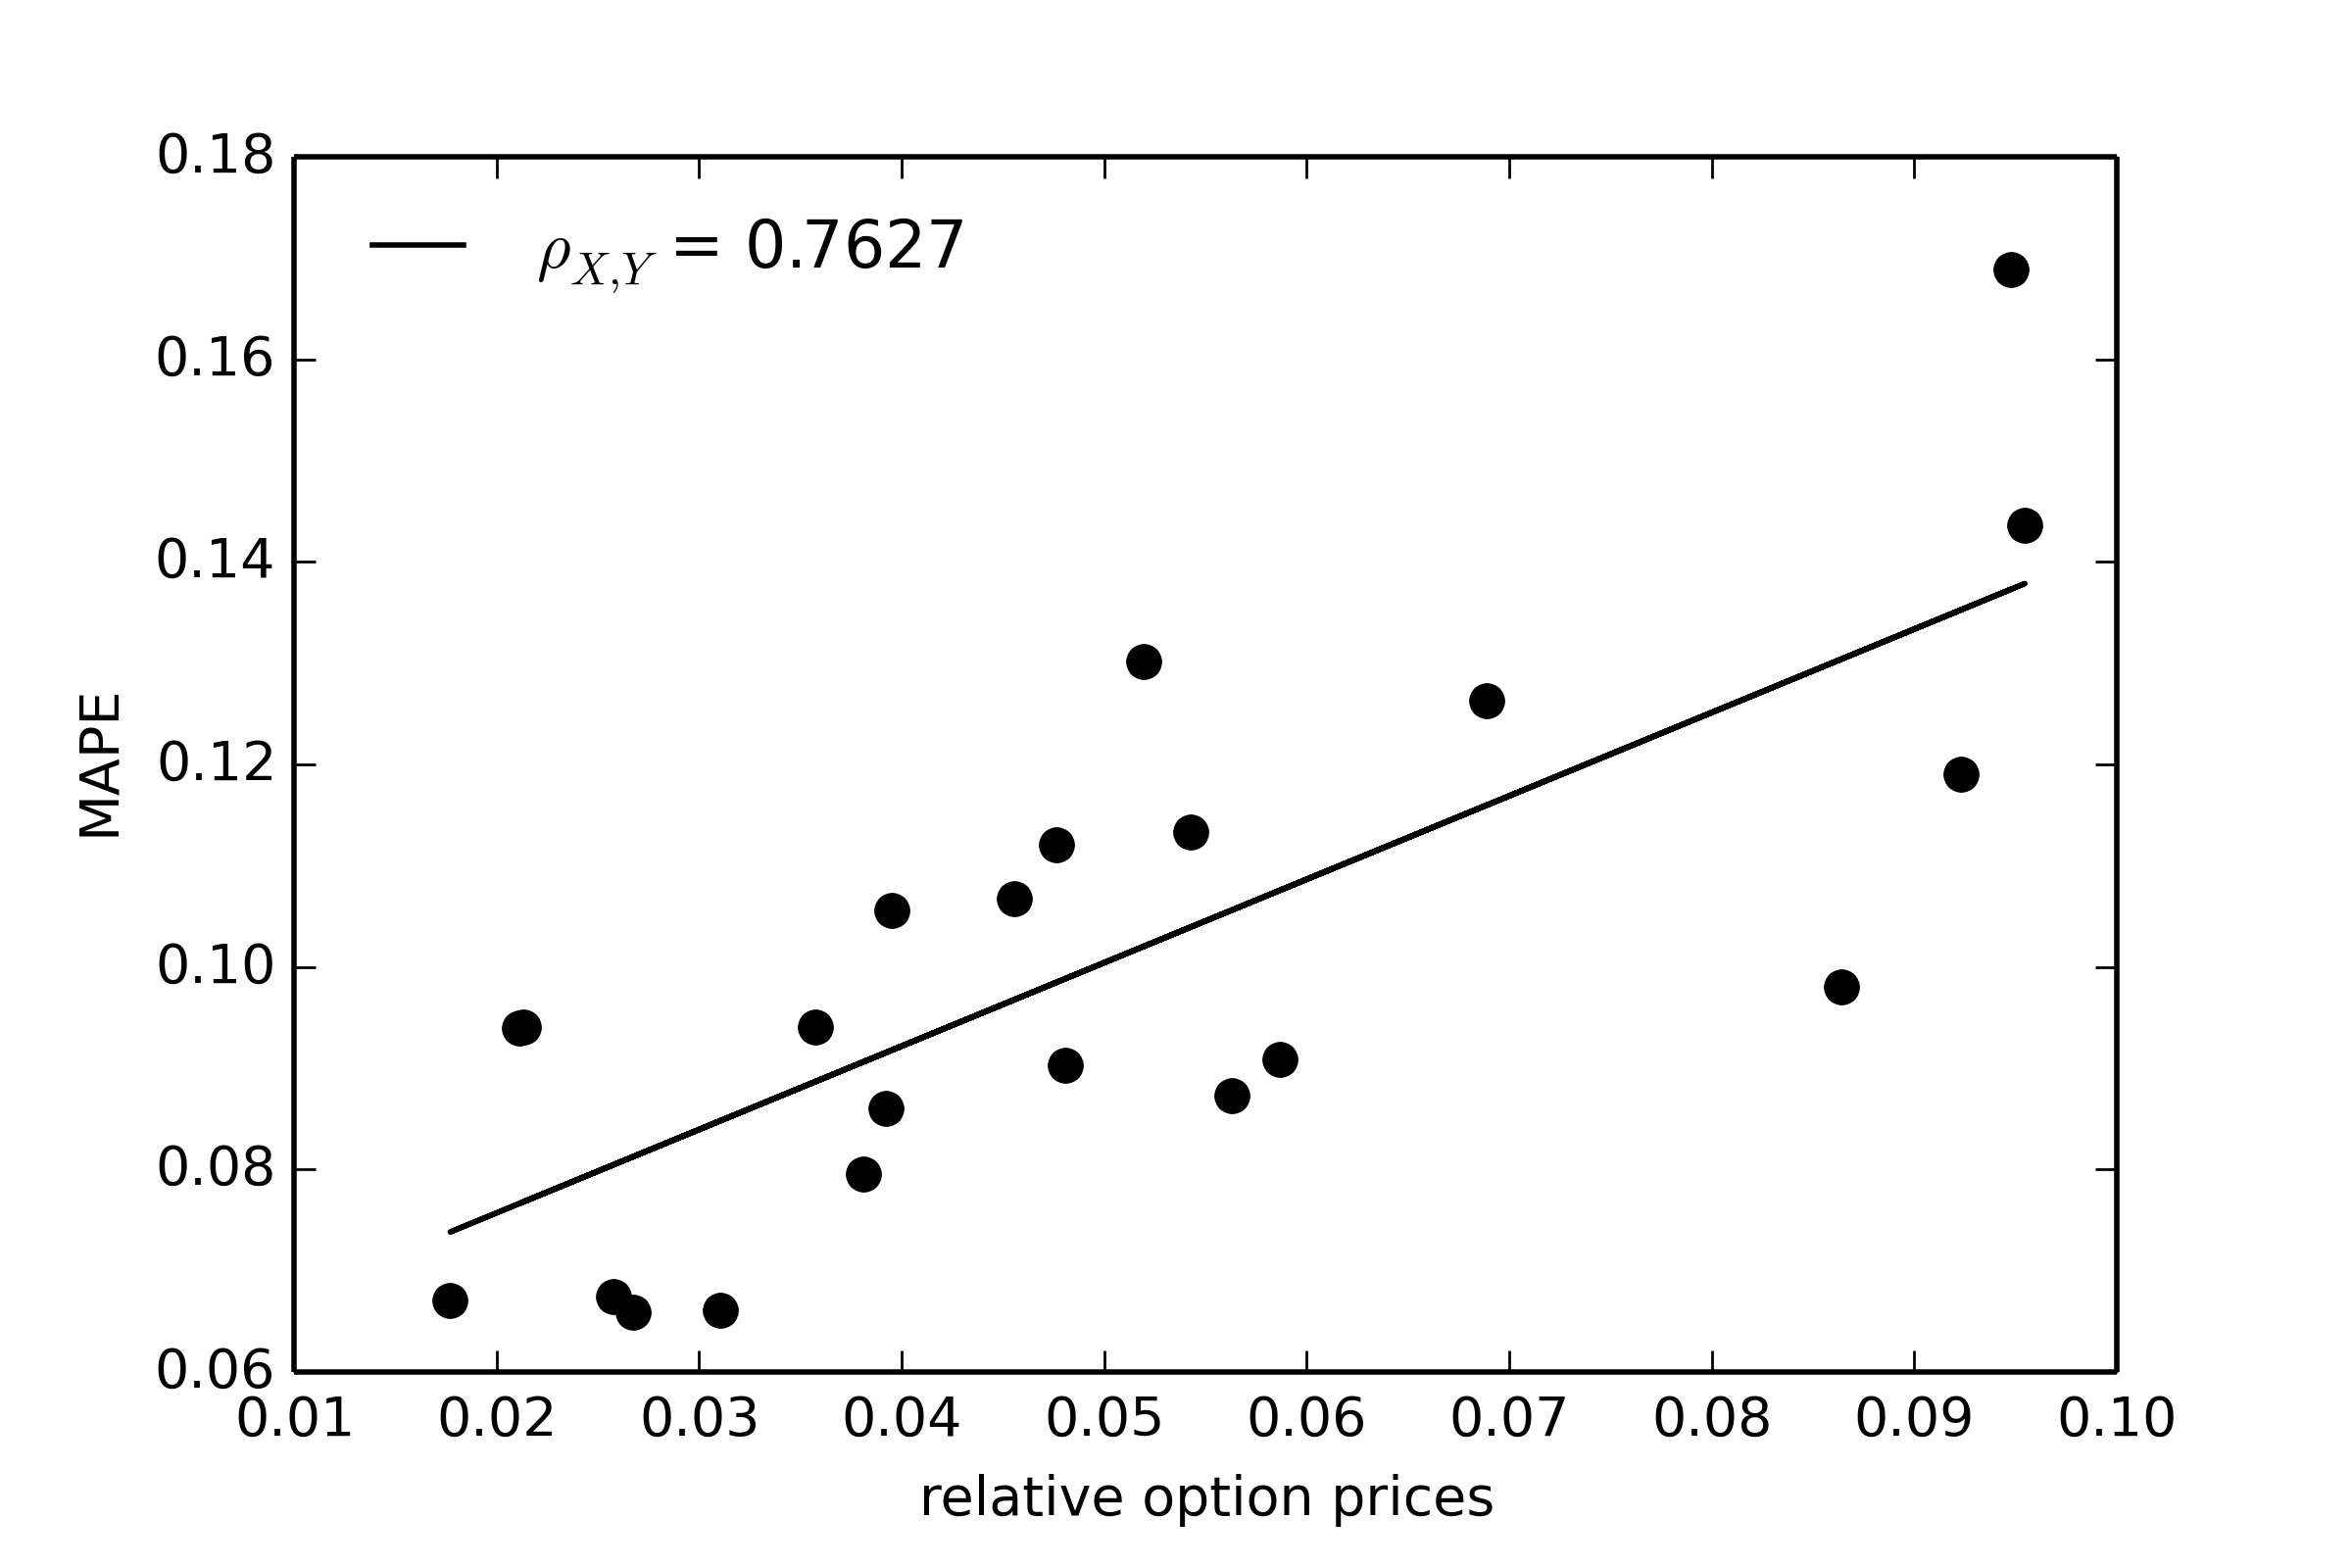
\includegraphics[width=0.8\textwidth]{figures/correlation_optionPrices-MAPE}
    \caption{Correlation between relative option prices and MAPE}
    \label{fig:optionPricesMAPE}
\end{figure*}


The results of this simulation model can be interpreted as the maximum profits possible in the current situation. Next section will alter some of the parameters and ascertain their influence on the gains the all knowing seller can receive.


\subsection{Sensitivity analysis}
After the first simulation, a sensitivity analysis is performed. For the base scenario, the all knowing option seller with foreknowledge will still be used. During the analysis only one of the parameters will be adjusted at a time. This way the exact effects of the variable can be examined.

The parameters for which a sensitivity analysis will be performed are \begin{inparaenum}[\itshape (i)\upshape]
    \item the options number of days till maturity,
    \item the passenger's risk parameter, and
    \item the passenger's likelihood of travelling.
\end{inparaenum}

\subsubsection{Option's number of days till maturity}
The first parameter for which a sensitivity analysis is performed is the number of days till maturity, $m$. In the base case, $m$ was set to 3~days, but this number will now be altered to values ranging from a 1~day till 21~days.

I expect the parameter $m$ to be of big influence on the realised profits of the option selling company. This is because the passenger is likely to make less accurate predictions because of the increasing time horizon. On the other hand, however, the option seller in this simulation still has foreknowledge. So, he does not have these increased uncertainties. This will likely create larger gaps between the passenger's WTP and the seller's WTA. Because the assumption is made that the seller knows the passenger's maximum WTP, he will be able to set higher option prices.

Next to this higher expected forecasting error, the option prices will also increase relative to its number of days till maturity, because of the higher probability of a big upward price motion.


\begin{figure*}
    \centering
    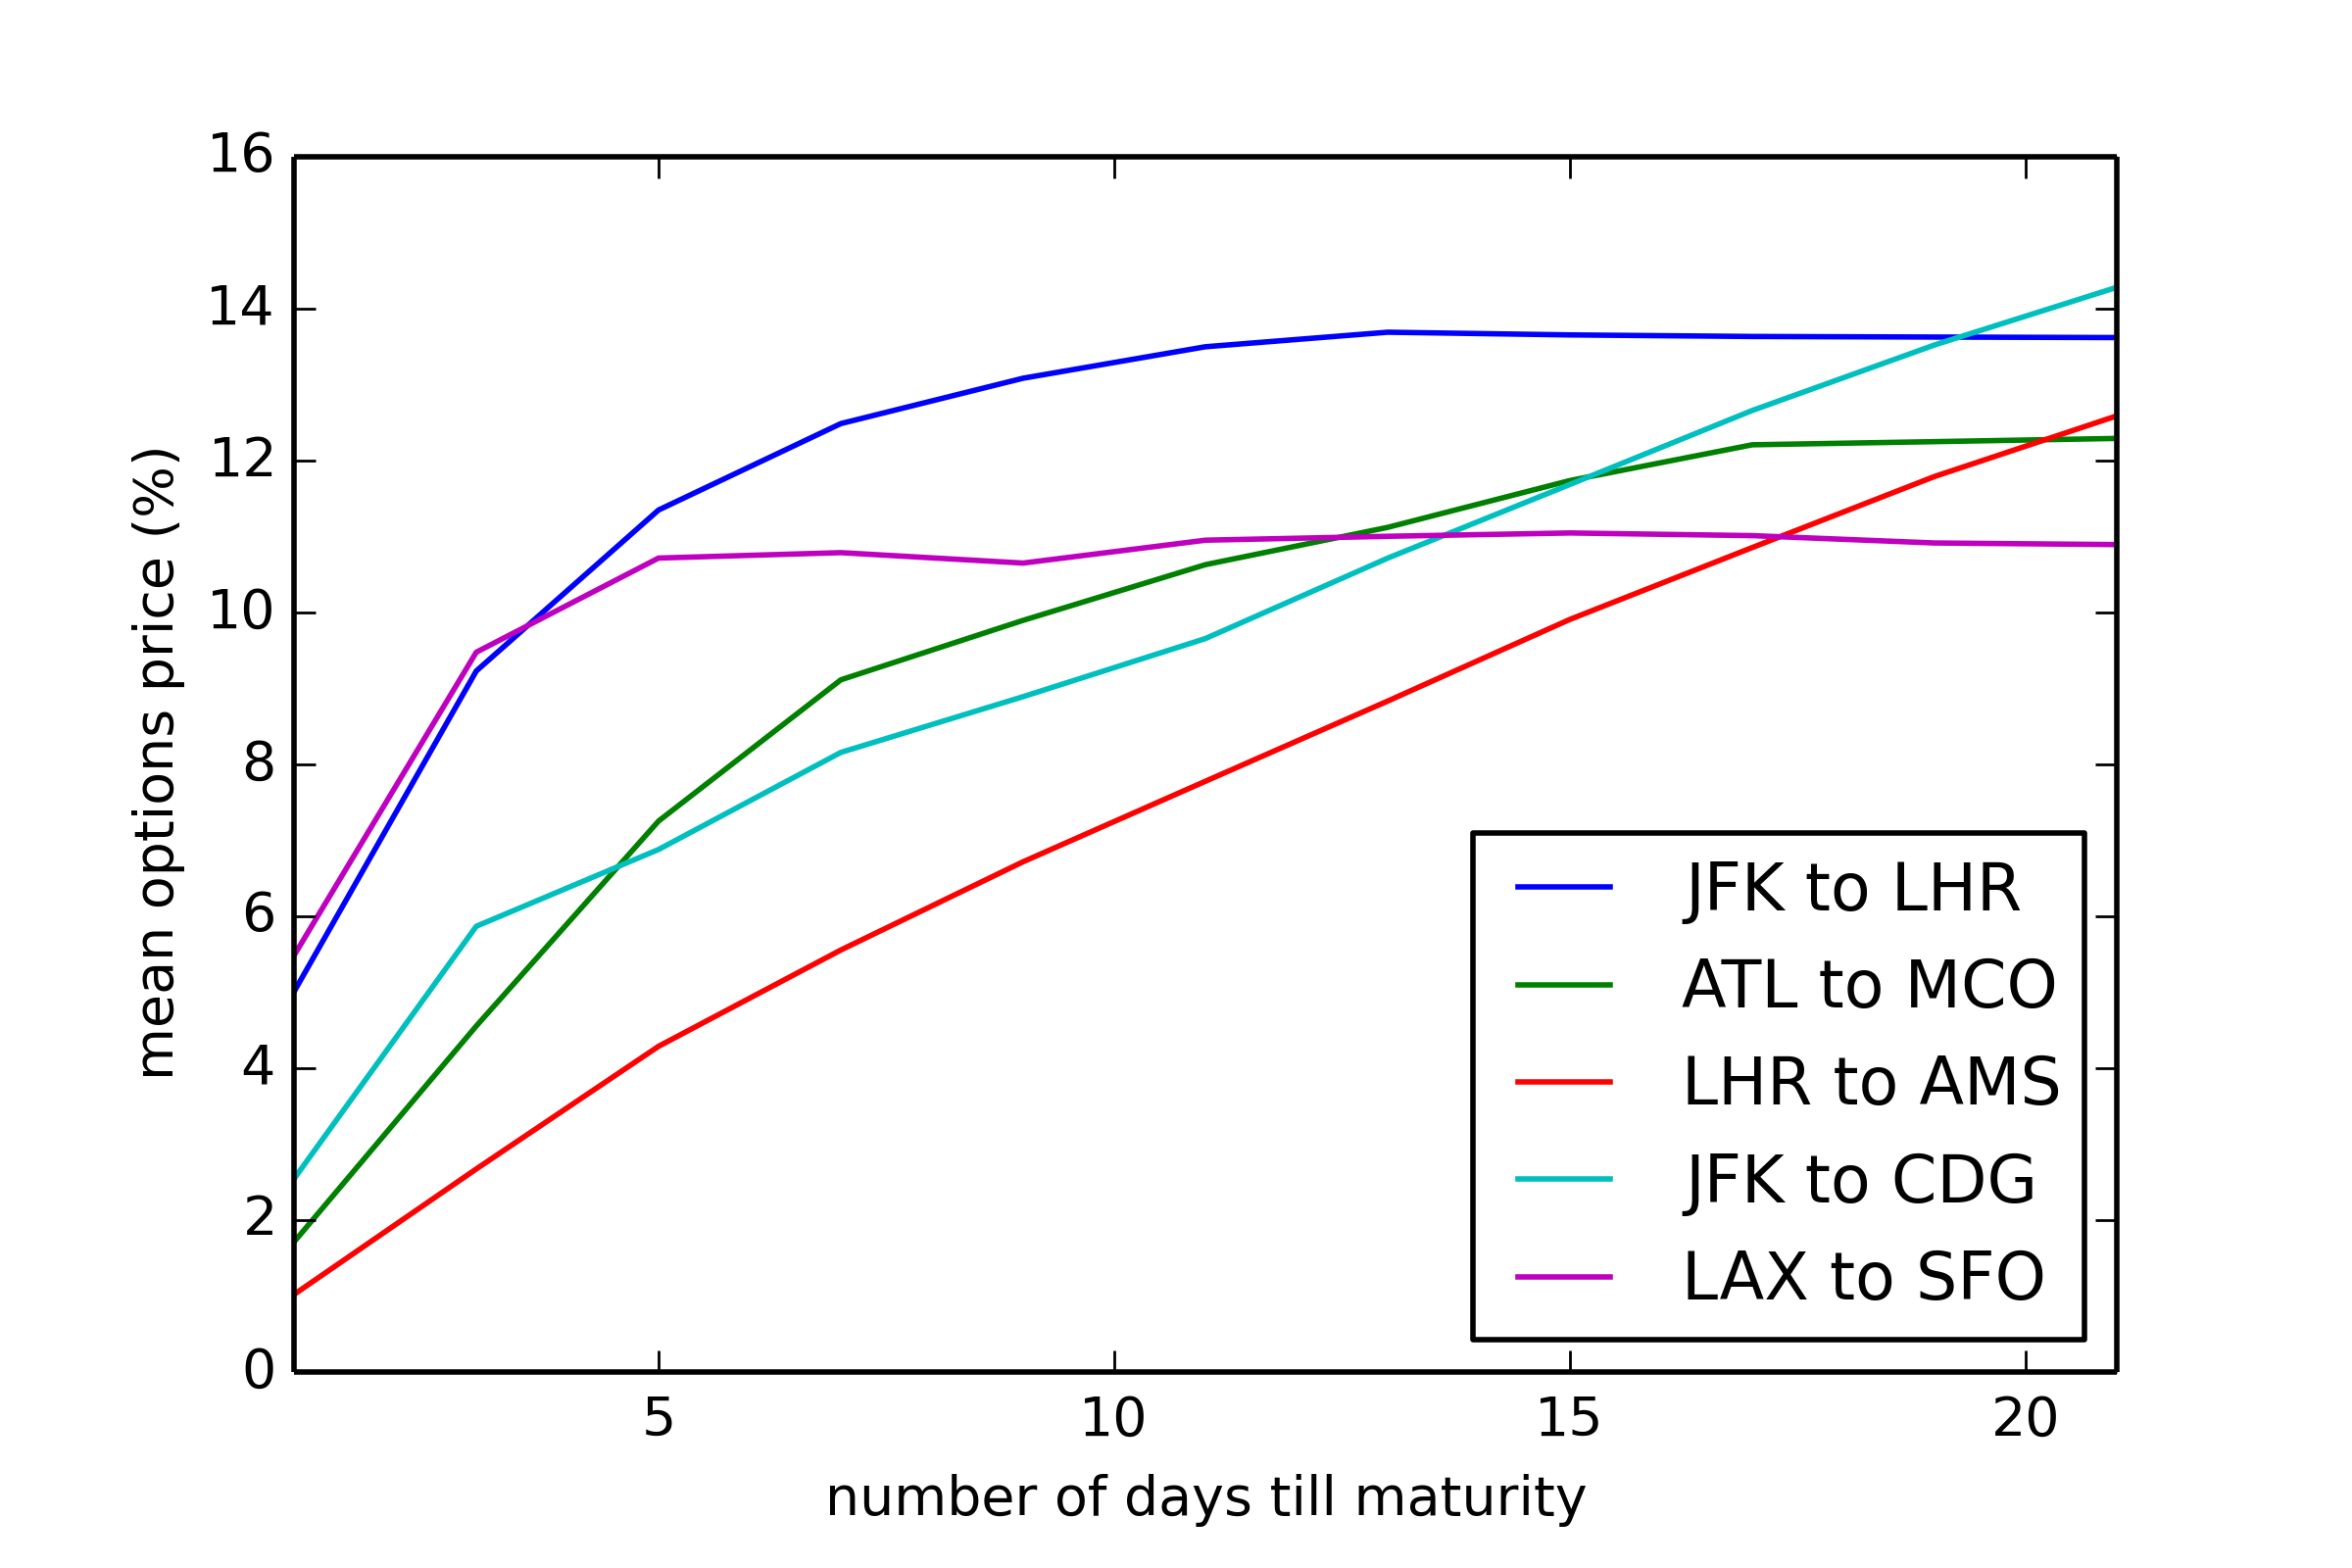
\includegraphics[width=0.8\textwidth]{figures/Sensitivity_maturity}
    \caption{Effect of number of days till maturity on relative option price}
    \label{fig:SensitivityMaturity}
\end{figure*}



\subsubsection{Passenger's risk parameter}

\subsubsection{Passenger's likelihood of travelling}



